\section{系统架构设计}

\subsection{总体架构}

系统按“表现层—接入层—AI 能力层—数据与外设层”组织。浏览器负责渲染、交互与状态；Next.js Route Handlers 负责鉴权、限流、参数校验、SSE 与 AI 调用；AI 能力层由 Agent、关系判定、混合检索、多模态与 MCP 组成；数据层保存账号、星空快照、问答历史、用量与缓存，并连接外部文献源和模型服务。

\begin{figure}[htbp]
\centering
\begin{tikzpicture}[font=\scriptsize,>=Latex,
  box/.style={draw=rule,fill=white,rounded corners=1.2mm,align=center,inner sep=1.8pt,minimum height=7mm},
  band/.style={draw=accent!18,fill=soft,rounded corners=2mm},
  lab/.style={font=\heiti\scriptsize,color=ink2,align=center}]

  % L1
  \node[lab,text width=0.95cm] (l1) at (0.65,8.4) {表现层};
  \node[box,text width=2.55cm] (b1) at (3.7,8.4) {页面与路由\\App Router};
  \node[box,text width=2.55cm] (b2) at (7.0,8.4) {Canvas 星图\\渲染管线};
  \node[box,text width=2.35cm] (b3) at (10.3,8.4) {Zustand\\跨组件状态};
  \node[box,text width=2.45cm] (b4) at (13.65,8.4) {问答面板\\SSE 消费};

  % L2
  \node[lab,text width=0.95cm] (l2) at (0.65,5.9) {接入层};
  \node[box,text width=2.55cm] (c1) at (3.7,5.9) {Route Handlers\\/api/*};
  \node[box,text width=2.35cm] (c2) at (7.0,5.9) {鉴权 / 限流\\预算控制};
  \node[box,text width=2.35cm] (c3) at (10.3,5.9) {Zod 校验\\安全护栏};
  \node[box,text width=2.45cm] (c4) at (13.65,5.9) {SSE / JSON\\文件流};

  % L3
  \node[lab,text width=0.95cm] (l3) at (0.65,3.45) {AI 能力层};
  \node[box,text width=2.15cm] (d1) at (2.95,3.45) {Agent\\规划 / 执行\\评估};
  \node[box,text width=2.15cm] (d2) at (5.7,3.45) {关系判定\\硬约束\\多标签判定};
  \node[box,text width=2.15cm] (d3) at (8.45,3.45) {混合 RAG\\BM25 + 向量\\RRF 融合};
  \node[box,text width=2.15cm] (d4) at (11.2,3.45) {多模态\\图像证据};
  \node[box,text width=2.15cm] (d5) at (13.95,3.45) {MCP\\9 个只读工具};

  % L4
  \node[lab,text width=0.95cm] (l4) at (0.65,0.65) {数据与外设};
  \node[box,text width=2.15cm] (e1) at (2.95,0.65) {PostgreSQL\\账号 / 星空\\历史};
  \node[box,text width=1.95cm] (e2) at (5.55,0.65) {Redis\\TTL / 节流};
  \node[box,text width=1.95cm] (e3) at (8.05,0.65) {data/\\媒体 / 缓存};
  \node[box,text width=2.05cm] (e4) at (10.55,0.65) {模型服务\\LLM / Embedding};
  \node[box,text width=2.35cm] (e5) at (13.45,0.65) {文献源\\OpenAlex / arXiv / S2};

  \begin{scope}[on background layer]
    \node[band,fit=(l1)(b4)] {};
    \node[band,fit=(l2)(c4)] {};
    \node[band,fit=(l3)(d5)] {};
    \node[band,fit=(l4)(e5)] {};
  \end{scope}

  \draw[->,thick,accent!65] (8.1,7.55) -- (8.1,6.75) node[midway,right,font=\tiny,color=muted] {HTTPS + SSE};
  \draw[->,thick,accent!65] (8.1,5.05) -- (8.1,4.30) node[midway,right,font=\tiny,color=muted] {内部调用};
  \draw[->,thick,accent!65] (8.1,2.50) -- (8.1,1.75) node[midway,right,font=\tiny,color=muted] {读写 / 调用};
\end{tikzpicture}
\caption{StellarLit 总体架构：浏览器、Route Handlers、AI 编排与数据外设四层。}
\label{fig:arch}
\end{figure}

架构有一条贯穿全局的约束：\textbf{依赖单向}。\code{types} 只定义数据契约，\code{lib} 只放纯逻辑，\code{components} 只消费 \code{features} 与 \code{lib}，\code{app} 负责组装；\code{server} 只能被 \code{app/api} 引用，绝不允许进入浏览器包。这条约束写进了 \code{eslint.config.mjs}，违反即构建失败。之所以用工具而不是靠文档，是因为“这次先这样、下次再拆”从来不会真的拆。

\begin{figure}[htbp]
\centering
\begin{tikzpicture}[font=\small,>=Latex,
  box/.style={draw=rule,fill=white,rounded corners=1.2mm,align=center,inner sep=3pt,minimum height=8mm},
  note/.style={draw=warm!45,dashed,fill=warm!4,rounded corners=1.2mm,align=center,inner sep=3pt}]
  \node[box,text width=2.0cm] (types) at (1.0,0) {\code{types}\\数据契约};
  \node[box,text width=2.2cm] (lib) at (4.1,0) {\code{lib}\\纯逻辑};
  \node[box,text width=2.6cm] (comp) at (7.4,0) {\code{components}\\展示与交互};
  \node[box,text width=2.2cm] (app) at (10.7,0) {\code{app}\\路由与组装};
  \node[box,text width=2.4cm] (server) at (4.1,-1.55) {\code{server}\\AI 接入与仓储};
  \node[box,text width=2.6cm] (api) at (10.7,-1.55) {\code{app/api}\\Route Handlers};

  \draw[->,thick,accent!65] (types) -- (lib);
  \draw[->,thick,accent!65] (lib) -- (comp);
  \draw[->,thick,accent!65] (comp) -- (app);
  \draw[->,thick,accent!65] (server) -- (api);
  \draw[->,thick,accent!65] (api) -- (app);
  \node[note,text width=8.6cm] at (7.4,-2.55) {ESLint 禁止反向依赖；密钥只存在于 \code{src/server}，不得进入浏览器包};
\end{tikzpicture}
\caption{分层与依赖方向：左侧永远不知道右侧存在，服务端代码不得进入浏览器包。}
\label{fig:deps}
\end{figure}

\needspace{3\baselineskip}
\subsection{技术选型与理由}

\begin{table}[htbp]
  \centering
  \footnotesize
  \caption{主要技术选型与取舍}
  \label{tab:stack}
  \begin{tabularx}{\textwidth}{L{2.5cm}L{4.2cm}Y}
    \toprule
\textbf{层} & \textbf{选型} & \textbf{为什么选它 / 代价是什么} \\
    \midrule
    框架 & Next.js 15（App Router）+ React 19 & 页面与 Route Handlers 同仓，AI 接入层不必另起服务；RSC 降低首屏数据往返。代价是构建内存较高，2G 机器需加 swap \\
    语言 & TypeScript strict & 图谱节点、边、模型输出都有明确契约；\code{unknown} 必须经过 Zod 才能进入业务 \\
    样式 & Tailwind CSS v4（CSS-first \code{@theme}） & 设计令牌即 CSS 变量，换主题等于换一套变量；避免样式与业务状态耦合 \\
    状态 & Zustand & 只有跨组件共享的状态才进 store；高频悬浮/选中不触发整树重渲染 \\
    渲染 & Canvas 2D 自写管线 & 上千节点/边时比 SVG/DOM 稳；绘制是纯函数，可脱离 React 测试。代价是命中检测要自己实现 \\
    数据库 & PostgreSQL 16（\code{pg} + JSONB） & 多账号并发写、事务与行级隔离；星空快照以 JSONB 保存，结构演进成本低 \\
    缓存 & Redis 7（\code{ioredis}） & TTL、跨实例共享、上游 host 节流；不可用时自动降级为进程内节流 \\
    校验 & Zod & 模型 JSON、API 入参、图像区域坐标共用一套 schema；解析失败可定位到字段 \\
    协议 & MCP TypeScript SDK & 复用官方工具注册与传输；HTTP 与 stdio 共用同一份工具定义 \\
    部署 & Docker Compose & 应用、PostgreSQL、Redis 一起编排；反向代理只负责 TLS 与 SSE 不缓冲 \\
    \bottomrule
  \end{tabularx}
\end{table}

\subsection{两条核心数据流}

系统有两条主链路：建图链路把“一篇种子”变成“一片星空”，问答链路把“一个问题”变成“一段带角标的回答”。两条链路共享同一份图谱数据契约与同一套模型配置，但在失败降级上各自独立：建图可以在没有模型时保留结构关系，问答在未绑定模型时明确提示，而不是静默给出不可信答案。

\begin{figure}[htbp]
\centering
\begin{tikzpicture}[font=\footnotesize,>=Latex,
  flowbox/.style={draw=rule,fill=white,rounded corners=1.2mm,align=center,inner sep=2.5pt,minimum height=8mm,text width=2.15cm},
  tag/.style={font=\heiti\scriptsize,color=accent2,anchor=west}]
  % build row
  \node[tag] at (-0.2,1.55) {建图};
  \node[flowbox] (s1) at (2.0,1.2) {种子输入\\标题/DOI/arXiv};
  \node[flowbox] (s2) at (4.55,1.2) {候选解析\\用户确认};
  \node[flowbox] (s3) at (7.1,1.2) {邻域展开\\向前/向后};
  \node[flowbox] (s4) at (9.65,1.2) {建图·聚类\\服务端布局};
  \node[flowbox] (s5) at (12.2,1.2) {关系判定\\证据核验};
  \node[flowbox] (s6) at (14.75,1.2) {持久化\\星图渲染};
  \foreach \a/\b in {s1/s2,s2/s3,s3/s4,s4/s5,s5/s6}
    \draw[->,thick,accent!60] (\a) -- (\b);

  % ask row
  \node[tag] at (-0.2,-1.35) {问答};
  \node[flowbox] (q1) at (2.0,-1.7) {问题 + 图像\\最多 4 张};
  \node[flowbox] (q2) at (4.55,-1.7) {安全护栏\\限流/预算};
  \node[flowbox] (q3) at (7.1,-1.7) {初始规划\\JSON 选工具};
  \node[flowbox] (q4) at (9.65,-1.7) {工具检索\\补查/扩展};
  \node[flowbox] (q5) at (12.2,-1.7) {覆盖判定\\确定性停止};
  \node[flowbox] (q6) at (14.75,-1.7) {流式回答\\角标/轨迹};
  \foreach \a/\b in {q1/q2,q2/q3,q3/q4,q4/q5,q5/q6}
    \draw[->,thick,accent2!65] (\a) -- (\b);
\end{tikzpicture}
\caption{建图与问答两条主链路：前者重结构与证据，后者重检索、补查与可解释停止。}
\label{fig:flows}
\end{figure}

\subsection{知识图谱数据模型}

图谱不是“节点和边的集合”这么简单。学术文献里存在三种性质完全不同的知识：客观引用事实、语义推断、算法派生。如果把三者塞进一张扁平表，大模型的幻觉和真实引用看起来一样可信，用户想核对时系统也无法回答“你凭什么这么说”。因此本模型按\textbf{可核验程度}分三层，而不是按业务模块分层。

\begin{table}[htbp]
  \centering
  \small
  \caption{三层图谱：生产者、可信度与视觉表达}
  \label{tab:layers}
  \begin{tabularx}{\textwidth}{L{1.5cm}L{4.4cm}L{3.2cm}Y}
    \toprule
\textbf{层} & \textbf{内容} & \textbf{生产者} & \textbf{可信度与视觉} \\
    \midrule
    L1 结构层 & 引用 \code{CITES}、作者 \code{AUTHORED_BY}、发表 \code{PUBLISHED_IN}、提及 \code{MENTIONS} & OpenAlex、arXiv、Semantic Scholar & 权威、可公开核验；极细引力线与星体标签 \\
    L2 语义层 & 基线、同期、思路类似、同任务异方法、扩展、结论矛盾 & 大模型 + 提示词工程 & 不能直接核验，但必须带原文证据；不同关系有固定线型与颜色 \\
    L3 派生层 & 社区、领域、潜在连接 & 标签传播 + 模块度、向量近邻、统计检验 & 全部可复算；缩小时以星团与星云浮现 \\
    \bottomrule
  \end{tabularx}
\end{table}

节点分实体节点与聚合节点。实体节点包括论文、作者、期刊/会议、概念与文本块；聚合节点（社区、领域）没有自己的数据，是算法对实体节点的分组结果，删掉不影响事实层。文本块 \code{chunk} 是 RAG 的检索单元，必须携带 \code{locator}（章节、段落序号或原文偏移），否则模型给出的引用无法回溯——界面上那些角标就会变成不可点击的装饰。

\begin{table}[htbp]
  \centering
  \small
  \caption{六类内置语义关系：硬约束、证据策略与视觉编码}
  \label{tab:relations}
  \begin{tabularx}{\textwidth}{L{2.0cm}L{2.2cm}L{4.3cm}L{2.4cm}Y}
    \toprule
\textbf{关系} & \textbf{关系族} & \textbf{硬约束} & \textbf{证据策略} & \textbf{视觉} \\
    \midrule
    基线 & 谱系 & 必须存在引用；年份差 $\le 8$ & 结构 + 原文 & 带方向实线，粒子表示流向 \\
    扩展 & 谱系 & 必须存在引用；年份差 $\le 10$ & 结构 + 原文 & 带方向实线 \\
    同期 & 对照 & 互不引用；年份差 $\le 2$ & 结构 & 虚线（平行但未交汇） \\
    思路类似 & 对照 & 标题+摘要 TF-IDF 相似度 $\ge 0.15$ & 原文 & 冷色实线 \\
    同任务异方法 & 对照 & 必须共享任务 & 原文 & 双色调对撞线 \\
    结论矛盾 & 冲突 & 必须共享任务 & 原文 & 全图唯一暖红色 \\
    \bottomrule
  \end{tabularx}
\end{table}

写入图之前会校验六条不变式：语义边至少一条证据；结构边必须有上游出处；引用边不得自环且 \code{CITES} 不允许成环；聚合节点不得作为引用端点；同一对节点同一关系只保留置信度最高的一条并合并证据；文本块必须有定位。违反即拒绝入库，而不是静默降级。

\subsection{渲染架构与语义缩放}

系统选择 Canvas 而不是 SVG/DOM，原因不是“Canvas 更酷”，而是节点与边一旦上千，DOM 方案的三类开销会同时出现：内存与样式重算随节点数线性增长；布局一动要做上千次样式计算；悬浮高亮要改上千个类名。Canvas 把这三类开销压成一次绘制调用，代价是要自己实现命中检测——但命中检测本来就带空间语义（命中半径随缩放变化、空白处需要吸附），DOM 的 \code{:hover} 帮不上忙。

三条性能约定贯穿渲染管线：布局在服务端算完，前端只做投影，主线程不跑 $O(n^2)$；悬浮/选中双写，渲染循环读 ref、React 读 state，高频状态不触发重渲染；动画按秒计算而不按帧计数，\code{dt} 上限 64ms，在 120Hz 屏与切标签页回来时都不失真。

\begin{table}[htbp]
  \centering
  \caption{语义缩放：缩放比例对应抽象层级}
  \label{tab:zoom}
  \begin{tabularx}{\textwidth}{L{2.6cm}L{3.2cm}Y}
    \toprule
\textbf{缩放区间} & \textbf{看到什么} & \textbf{读的是哪一层} \\
    \midrule
    \code{scale < 0.34} & 领域星云 + 中文标题 & \code{domain} 聚合节点 \\
    \code{0.34 <= scale < 0.78} & 星团 + 社区标签 & \code{community} 聚合节点 \\
    \code{scale >= 0.78} & 论文星体 + 关系边 & \code{paper} 实体节点与边 \\
    \bottomrule
  \end{tabularx}
\end{table}

增量构建是“星空会长大”的关键。新增种子时，如果整张图重新布局，老星体会整体漂移，用户看到的现象就是“我一搜，原来的星图就没了”。因此世界原点固定在中心，世界只做对称长大；已有节点作为锚点被拉回原位，新节点先插到已有邻居的重心附近再自由松弛，老星体的绝对坐标一个都不动。社区重聚类后，再按新旧社区的重叠票数做编号对齐，让大部分论文保持原来的社区编号。

\begin{figure}[htbp]
  \centering
  \begin{minipage}{0.49\textwidth}
    \centering
    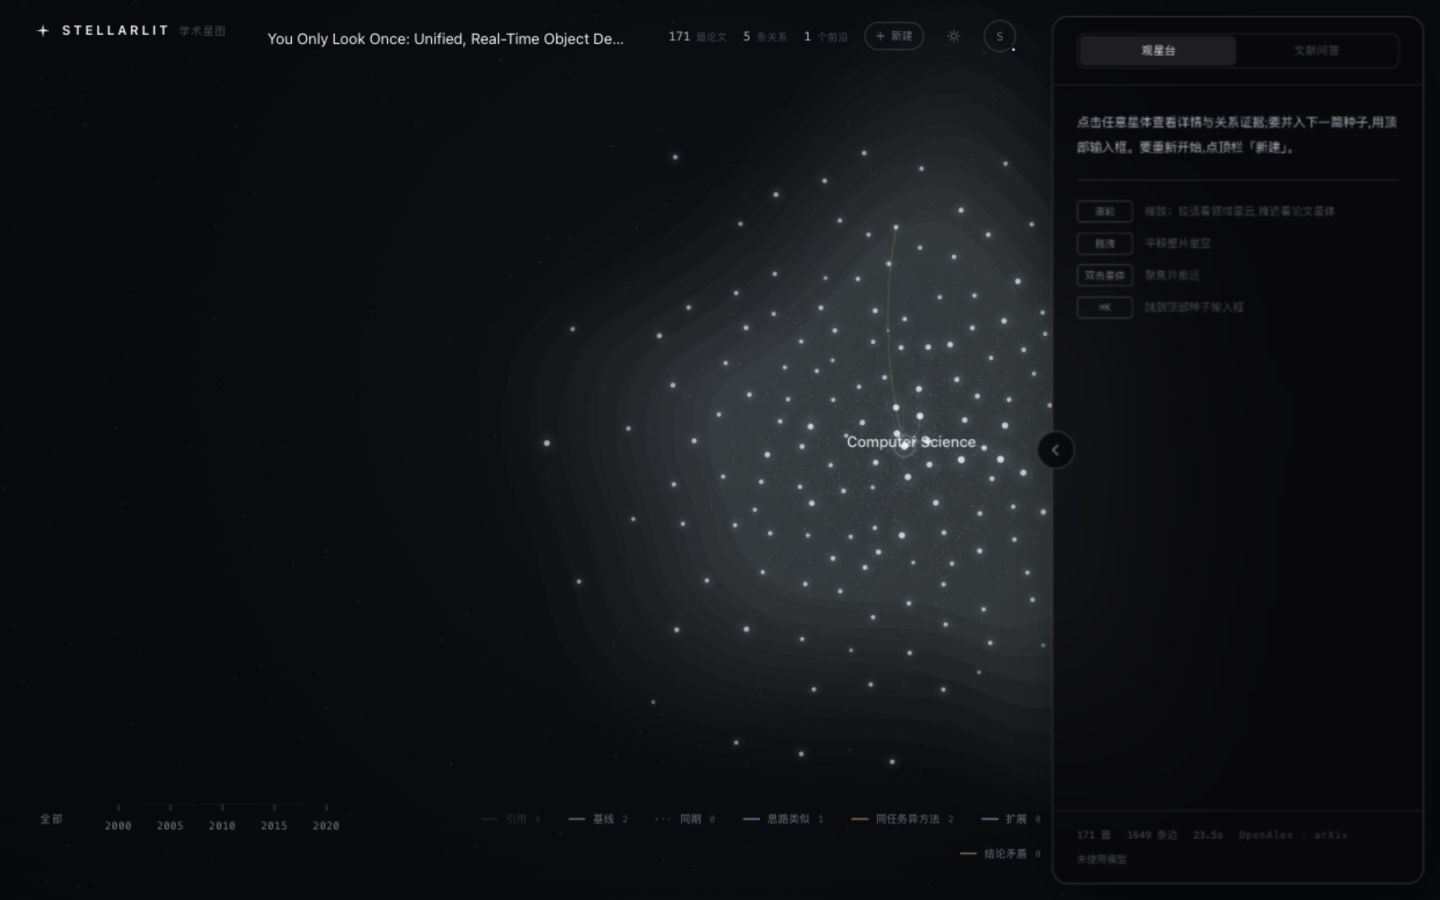
\includegraphics[width=\linewidth]{01-starfield.png}
    \caption{星图画布：拉远是领域星云，推近是论文星体。}
    \label{fig:starfield}
  \end{minipage}\hfill
  \begin{minipage}{0.49\textwidth}
    \centering
    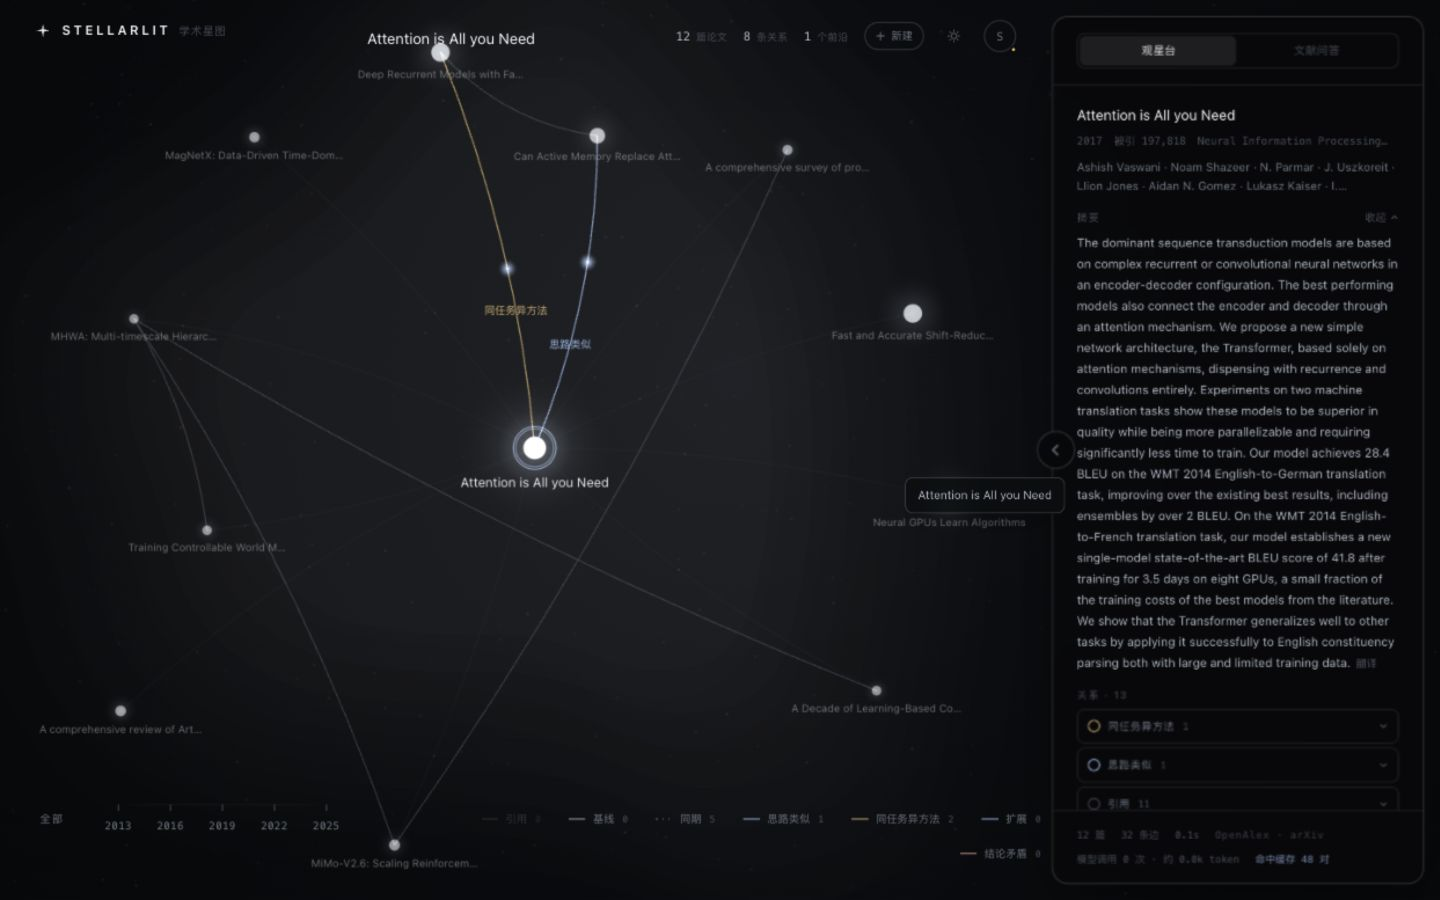
\includegraphics[width=\linewidth]{02-evidence.png}
    \caption{论文详情与关系证据：每条边可点回原文片段。}
    \label{fig:evidence}
  \end{minipage}
\end{figure}
